\documentclass[12pt]{article}
\usepackage{minted}
\usepackage{graphicx}
\usepackage{mathtools}
\usepackage{amsfonts}

\begin{document}
    \title{CS 541 Homework 3}
    \author{Stephen Szemis}
    \date{November 7, 2020}
    \maketitle

    \paragraph{Part 1: Gradient Calculation}~\\
    Let's start with the initial Sigmoid Function.
    \[
        F(w) = \frac{1}{(1 + e^{-x \cdot w})}
    \]
    Let's write it without the negatives. It's simple manipulation.
    \[
        F(w) = \frac{1}{(1 + e^{-x \cdot w})} * 
        \frac{e^{x \cdot w}}{e^{x \cdot w}} = 
        \frac{e^{x \cdot w}}{e^{x \cdot w} + 1}
    \]
    Now let's begin our gradient. First we can use the product rule.
    \[
        \nabla F(w) = 
        ( \nabla e^{x \cdot w} * \frac{1}{e^{x \cdot w} + 1} )
        + ( e^{x \cdot w} * \nabla \frac{1}{e^{x \cdot w} + 1} )
    \]
    Simplified down some of the easier derivatives.
    \[
        \nabla F(w) = 
        \frac{e^{x \cdot w}}{e^{x \cdot w} + 1}
        + ( e^{x \cdot w} * \nabla \frac{1}{e^{x \cdot w} + 1} )
    \]
    So now we need the gradient of that fraction. Lets use the chain rule.
    \[
        \nabla \frac{1}{e^{x \cdot w} + 1} =
        -(e^{x \cdot w} + 1)^{-2} * (e^{x \cdot w} + 0)
    \]
    Easy enough. Now let's plug that back into our large equation and we get\dots
    \[
        \nabla F(w) = 
        \frac{e^{x \cdot w}}{e^{x \cdot w} + 1} +
        ( e^{x \cdot w} * -(e^{x \cdot w} + 1)^{-2} * e^{x \cdot w} ) =
        \frac{e^{x \cdot w}}{e^{x \cdot w} + 1} -
        (\frac{e^{x \cdot w}}{e^{x \cdot w} + 1})^{2}
    \]
    Pull out some stuff.
    \[
        \nabla F(w) =
        \frac{e^{x \cdot w}}{e^{x \cdot w} + 1} *
        ( 1 - \frac{e^{x \cdot w}}{e^{x \cdot w} + 1}) =
        F(w) * (1 - F(w))
    \]
    And there you have it.

    \noindent Now let's do the logistic function.
    \[
        F(w) = log(1 + e^{-yx \cdot w})
    \]
    Again we will need to use the chain rule. So let's define the the two gradients we need.
    First the outer gradient.
    \[
        \nabla log(z) = \frac{1}{z} = \frac{1}{1 + e^{-yx \cdot w}}
    \]
    And the inner gradient.
    \[
        \nabla (1 + e^{-yx \cdot w}) = 0 - ye^{-yx \cdot w}
    \]
    Using those in our chain rule we get\dots
    \[
        \nabla F(w) = \frac{1}{1 + e^{-yx \cdot w}} * (-ye^{-yx \cdot w})
    \]
    This can be simplified down.
    \[
        \nabla F(w) = 
        -y * \frac{1}{1 + e^{-yx \cdot w}} * \frac{1}{e^{yx \cdot w}} =
        \frac{-y}{e^{yx \cdot w} + 1}
    \]
    And that is that, I think.

    \paragraph{Part 2: Linear Regression}
    \subparagraph{1. Gradient, Hessian, and Convexity}~\\
    We have (1) define below.
    \[
        F(w) = \frac{1}{2} \| y - Xw \|^{2}_{2}
    \]
    We can expand the l2-norm out as the following vector / matrix operations.
    \[
        F(w) = \frac{1}{2} (y - Xw)^{T}(y - Xw)
    \]
    Expand out.
    \[
        F(w) = \frac{1}{2} (y^{T}y - y^{T} X w + w^{T} X^{T} X w - y X^{T} w^{T})
    \]
    Simply down.
    \[
        F(w) = \frac{1}{2} y^{T}y - w^{T} X^{T} y + \frac{1}{2} w^{T} X^{T} X w
    \]
    Now take the gradient with respect to w.
    \[
        \nabla F(w) = -X^{T}y + X^{T} X w 
    \]
    If we want the Hessian, we can now take the second partial with respect to w.
    \[
        \nabla^{2} F(w) = X^{T} X
    \]
    And we are done. Now let's show that it is convex. It is known that if the Hessian is a 
    positive semi-definite then the original function is convex. We can see that \(X^{T} X\) 
    since if \(X\) contains only real values (which is does by the problem definition) \(X^{T} X\)
    must be semi-positive definite.

    \subparagraph{2. Equivalence}~\\
    We use the least-squares formulation because least squares is smooth, while (2) is not.
    So it is easier to find the true global optimum of (1) then it is for (2).

    \subparagraph{3. Strongly-Convex}~\\
    In order to force F to be strongly-convex we must make it's Hessian more then just semi-positive definite
    , instead it must be positive definite. One way to do this is make X be a symmetric matrix, since then
    \(X^{T}X\) will always be a strictly positive matrix, which in turn guarantees a strongly-convex function.

    \subparagraph{4. Coding Problem}
    The code for these next two parts is found after as final section of homework.

    As you can see from these graphs, we see a fast improvement towards convergence with the 
    optimum, until we multiply by 20 or 100. At that point, we massively overshoot our values and get
    strange unexpected behavior. We can see that 2 seems to be the max value we can increase our mu by.
    This is in line with our theory that 2/(alpha + L) is max when dealing with strongly convex functions, 
    it's possible our random matrix X is almost symmetric, giving an almost optimal behavior with this 
    mu.
    \begin{center}
    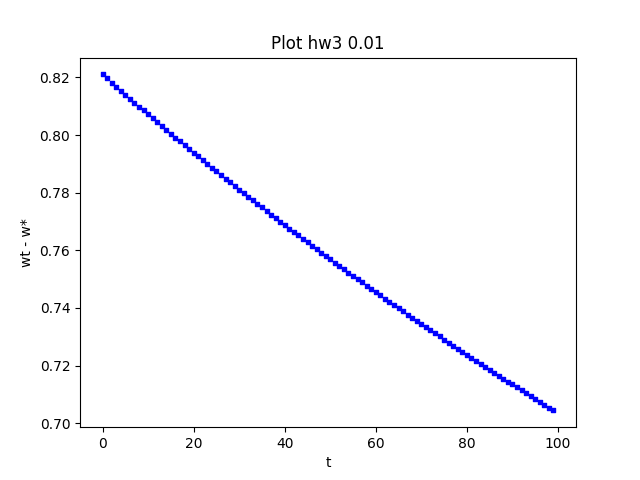
\includegraphics[width=5cm]{part 4/Figure_1.png}
    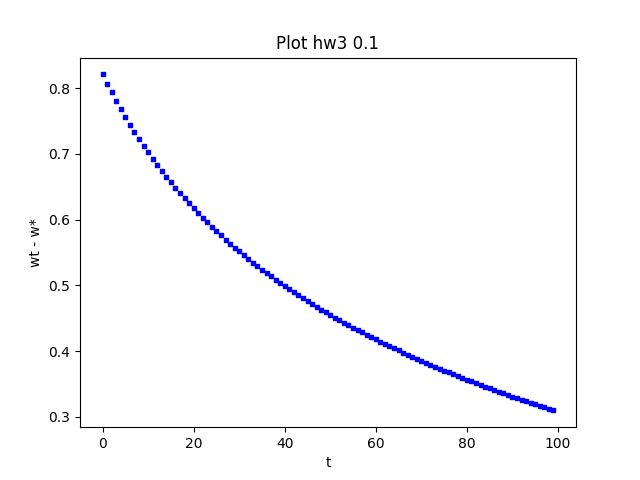
\includegraphics[width=5cm]{part 4/Figure_2.png}
    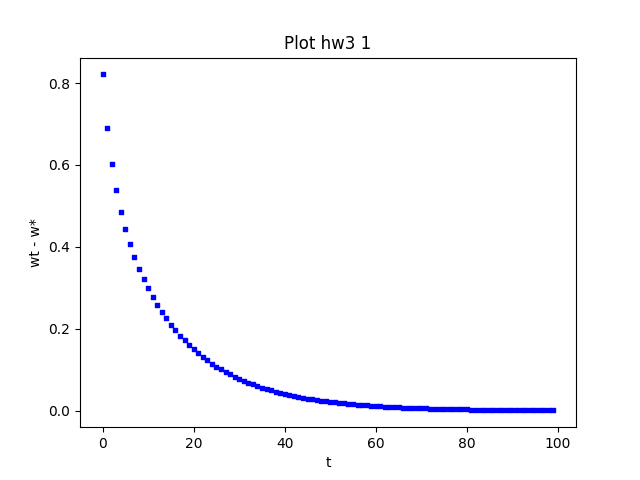
\includegraphics[width=5cm]{part 4/Figure_3.png}
    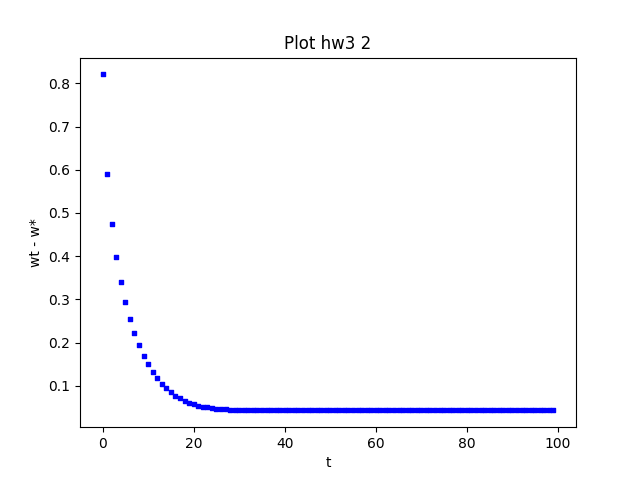
\includegraphics[width=5cm]{part 4/Figure_4.png}
    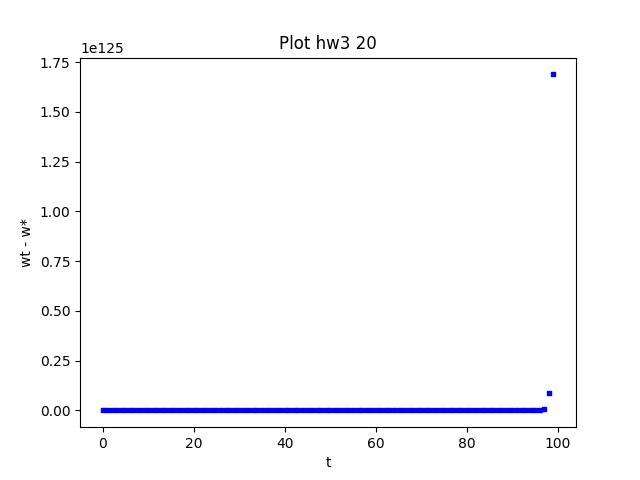
\includegraphics[width=5cm]{part 4/Figure_5.png}
    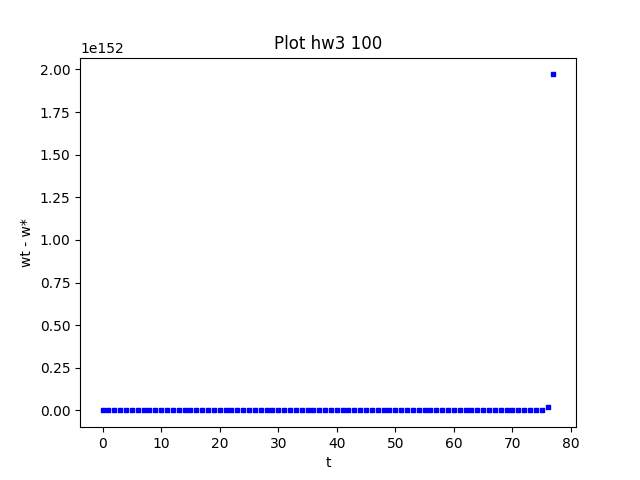
\includegraphics[width=5cm]{part 4/Figure_6.png}
    \end{center}

    \subparagraph{5. Coding Problem}
    We use similar code for both sections, simply change values of n and d and also used 
    our function diff1 instead of diff. See code below.

    \begin{center}
    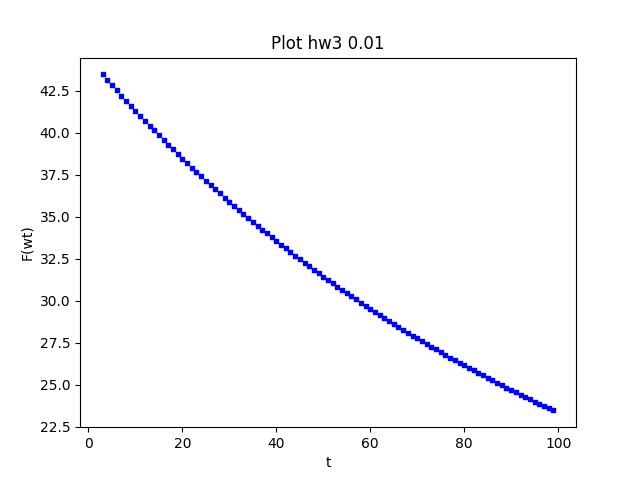
\includegraphics[width=5cm]{part 5/Figure_1.png}
    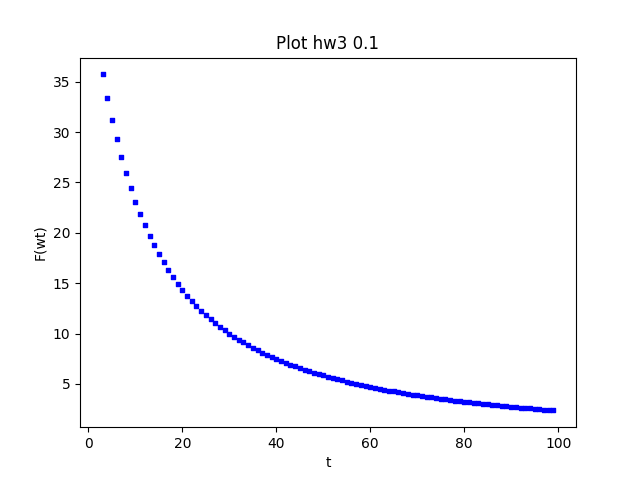
\includegraphics[width=5cm]{part 5/Figure_2.png}
    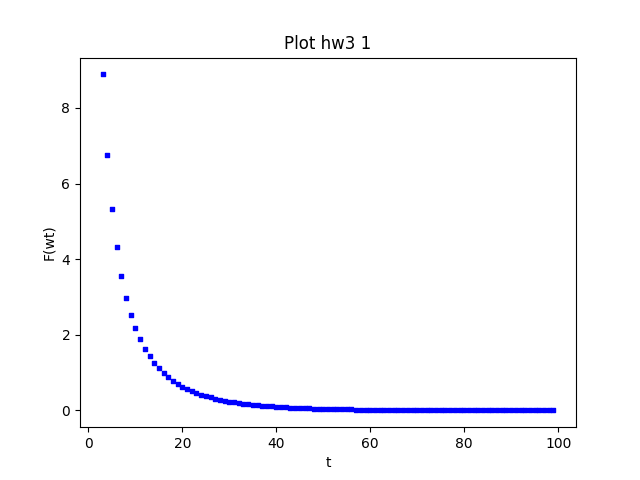
\includegraphics[width=5cm]{part 5/Figure_3.png}
    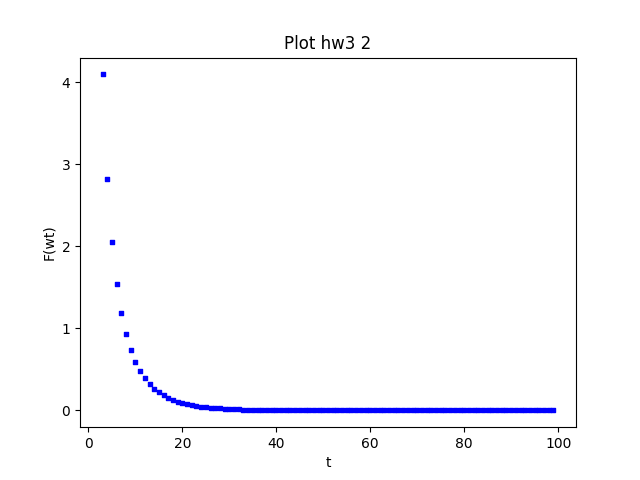
\includegraphics[width=5cm]{part 5/Figure_4.png}
    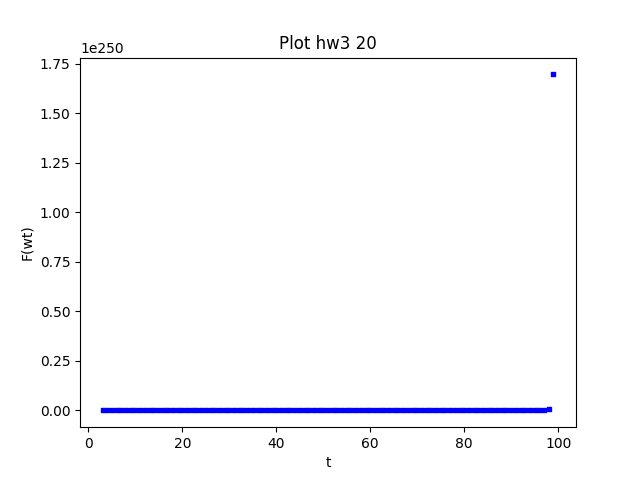
\includegraphics[width=5cm]{part 5/Figure_5.png}
    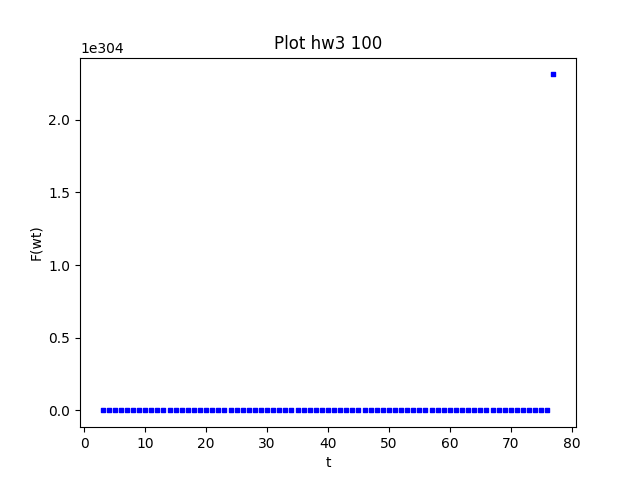
\includegraphics[width=5cm]{part 5/Figure_6.png}
    \end{center}

    \inputminted{python}{Szemis_hw3.py}

\end{document}